\subsection{Computation of derivatives}\label{sec:derivatives}
Computation of derivative quantities such as gradient and Laplacian is of fundamental importance in
data analysis. Since simulation data can rarely be captured by closed-form formulas, we use finite
differences. In this section, we use 32 bits (instead of 16) for quantization, to ensure enough
precision for finite differences. We always perform finite differences on the finest (original)
resolution. This decision avoids the problem of computing distances between quantities defined on
grids of different sizes, because we are unaware of any widely accepted solutions to this problem.
\cref{sec:gradient} discusses gradient computation, and \cref{sec:laplacian} discusses
computation of the Laplacian.

\subsubsection{Gradient}\label{sec:gradient}

\begin{figure}[h]
	\centering
	\subcaptionbox{\emph{boiler}}{
	{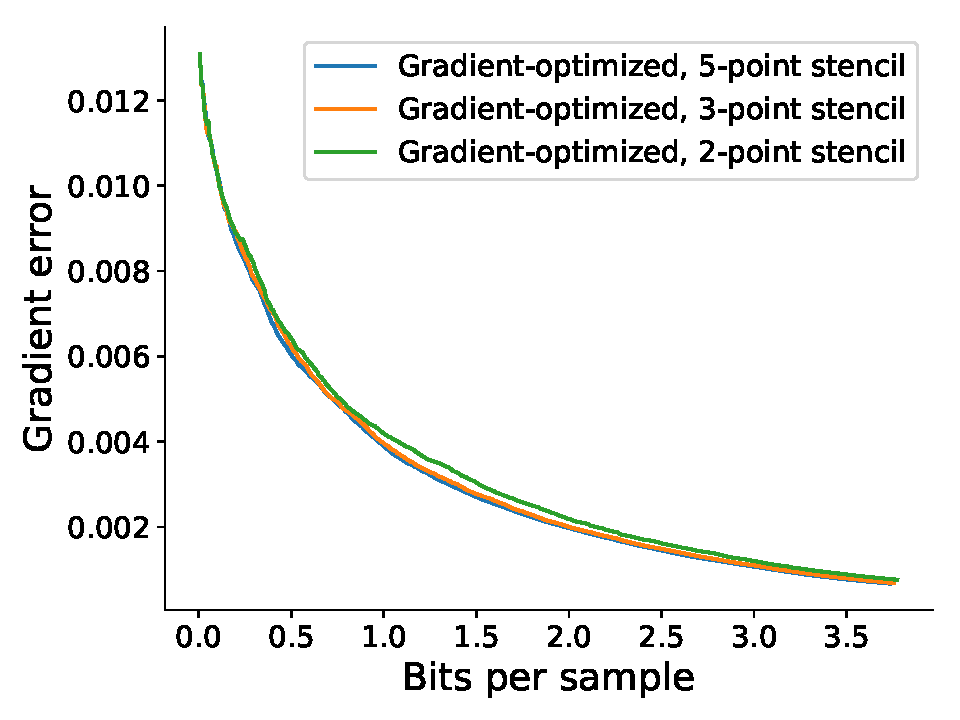
\includegraphics[width=0.48\linewidth]{gradient/gradient-optimized-boiler}}}
	\subcaptionbox{\emph{diffusivity}}{
	{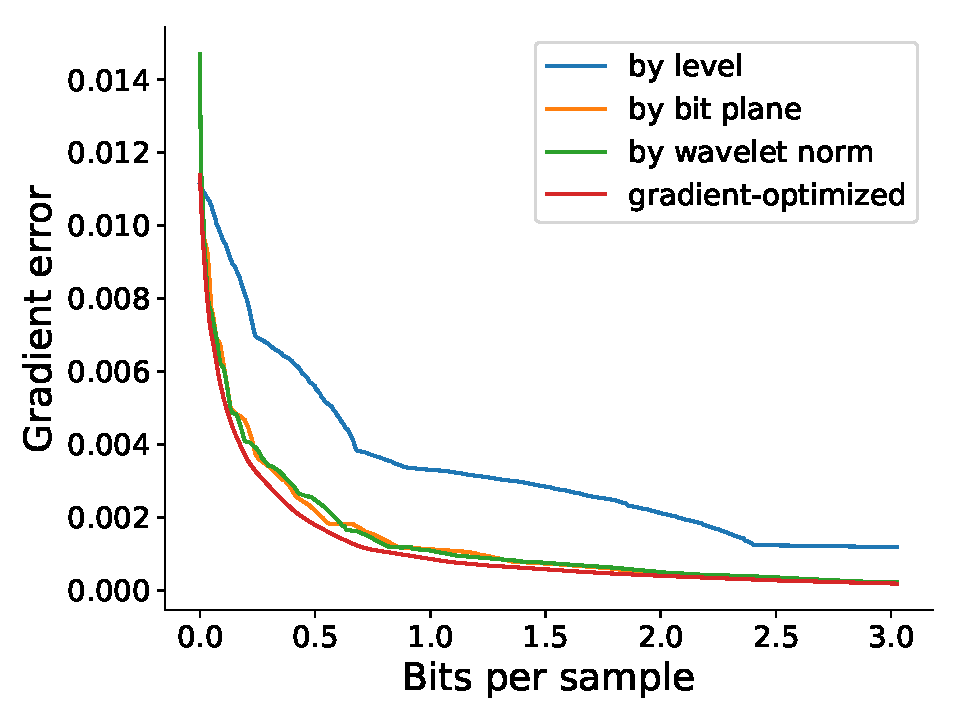
\includegraphics[width=0.48\linewidth]{gradient/gradient-optimized-diffusivity}}}
	\subcaptionbox{\emph{turbulence}}{
	{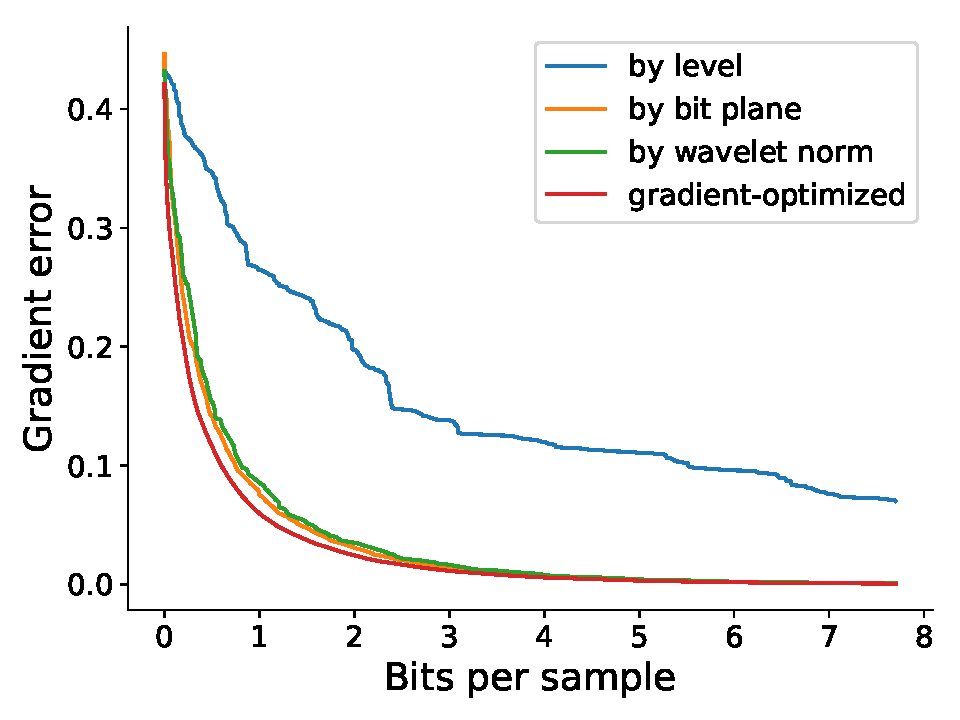
\includegraphics[width=0.48\linewidth]{gradient/gradient-optimized-turbulence}}}
	\subcaptionbox{\emph{pressure}}{
	{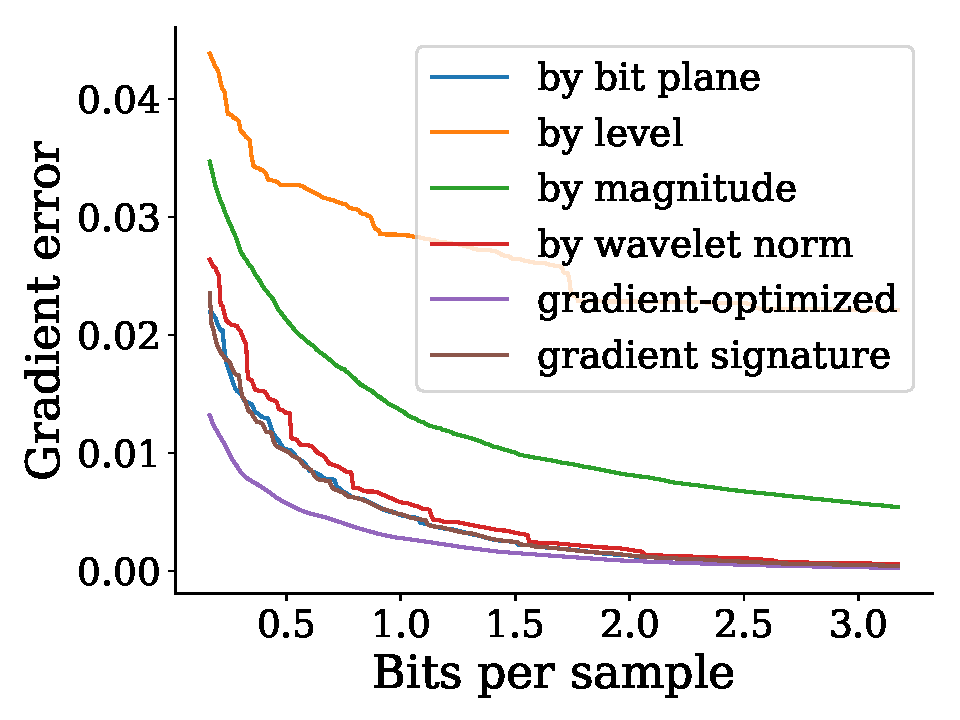
\includegraphics[width=0.48\linewidth]{gradient/gradient-optimized-pressure}}} \caption{Gradient
	error of reconstructed functions. Lower is better. Leading zero packets are removed, and the plots
	are truncated in the same way as in Figure \ref{fig:rmse-optimized}. The trend, in all cases, is
	$s_{grad-opt} > s_{grad-sig} \approx s_{bit} > s_{wav} > s_{mag} > s_{lvl}$.}
	\label{fig:gradient-error-comparison}
\end{figure}

\begin{figure}[h]
	\centering
	\subcaptionbox{\emph{by bit plane} ($s_{bit}$)}{
	{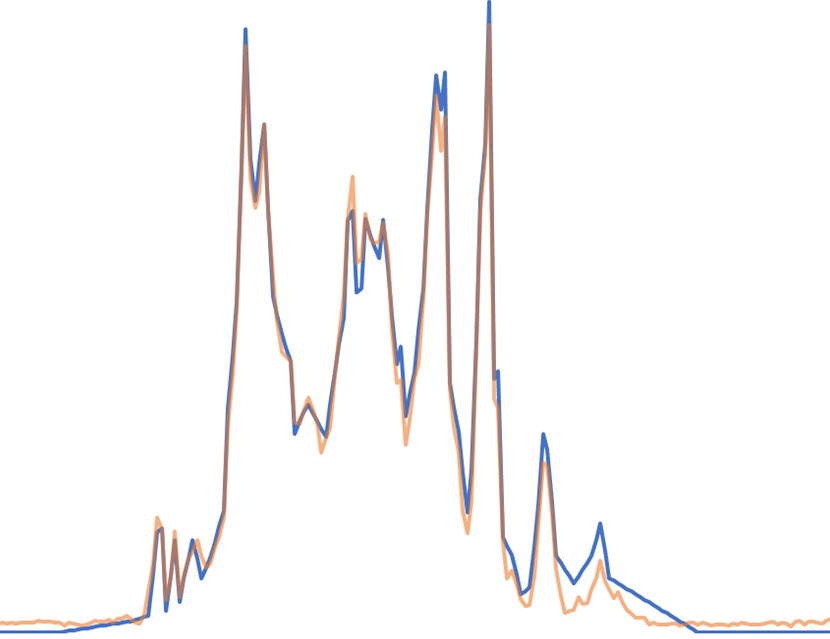
\includegraphics[width=0.48\linewidth]{gradient/gradient-bit-plane}}}
	\subcaptionbox{\emph{by wavelet norm} ($s_{wav}$)}{
	{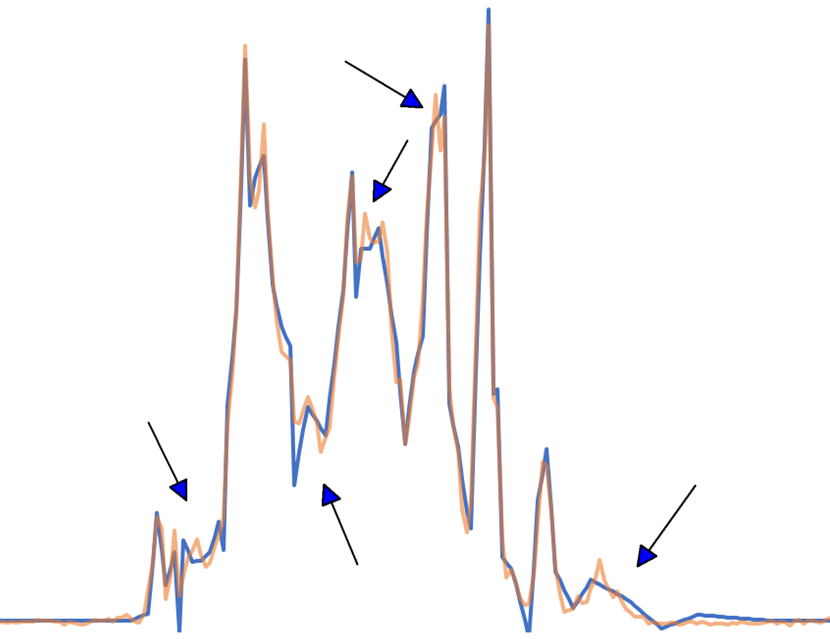
\includegraphics[width=0.48\linewidth]{gradient/gradient-wavelet-norm}}}
	\caption{A 1D line extracted from \emph{plasma}, and reconstructed using $s_{bit}$ and $s_{wav}$ at
	0.6 bps. The original data is in orange, whille the reconstructions are in blue. $s_{wav}$ captures
	well the function values in low-gradient regions, where $s_{bit}$ struggles (red arrows).
	However, $s_{bit}$ retains the shape of the original function well in areas of both low and high
	gradients, where $s_{wav}$ instead produces smooth approximations (blue arrows). $s_{bit}$
	therefore is better for	derivative computations, where a function's shape (or its relative
	values), matter more than its absolute values.}\label{fig:bit-plane-vs-wavelet-norm-gradient}
\end{figure}

\begin{figure}[h]
	\centering
	\subcaptionbox{\emph{by level} ($s_{lvl}$)}{
	{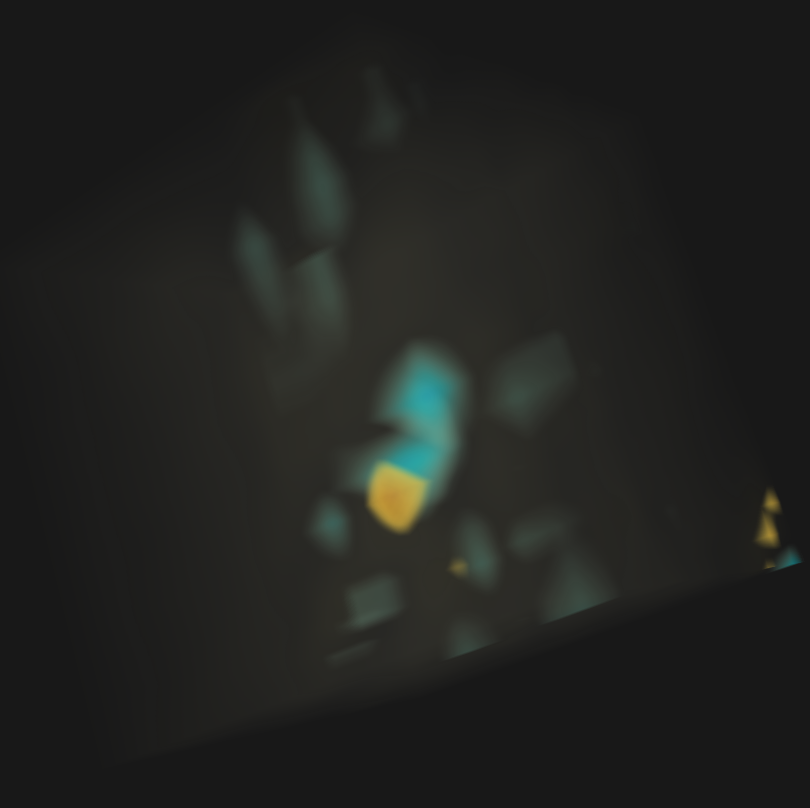
\includegraphics[width=0.31\linewidth]{gradient/gradient-turbulence-level}}}
	\subcaptionbox{\emph{by bit plane} ($s_{bit}$)}{
	{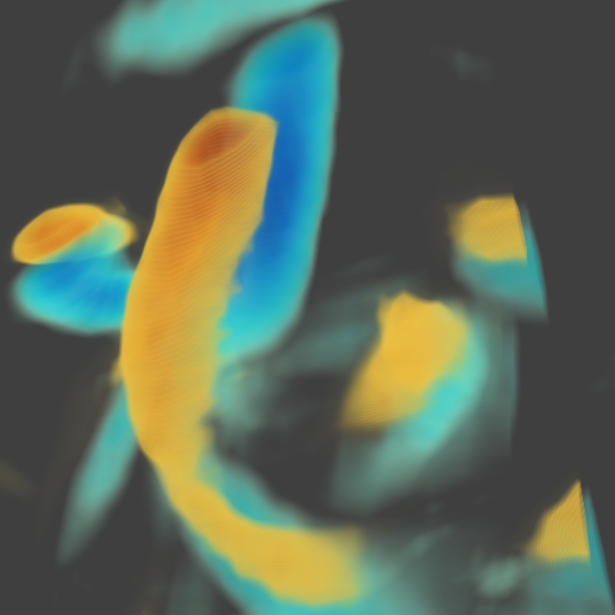
\includegraphics[width=0.31\linewidth]{gradient/gradient-turbulence-bit-plane}}}
	\subcaptionbox{\emph{by wavelet norm} ($s_{wav}$)}{
	{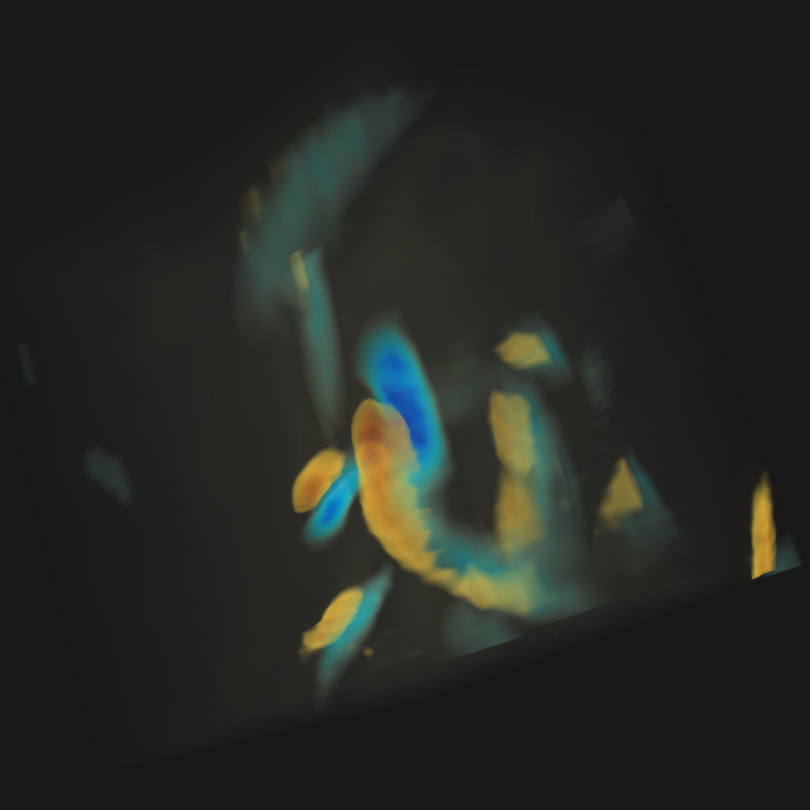
\includegraphics[width=0.31\linewidth]{gradient/gradient-turbulence-wavelet-norm}}}
	\subcaptionbox{\emph{by magnitude} ($s_{mag}$)}{
	{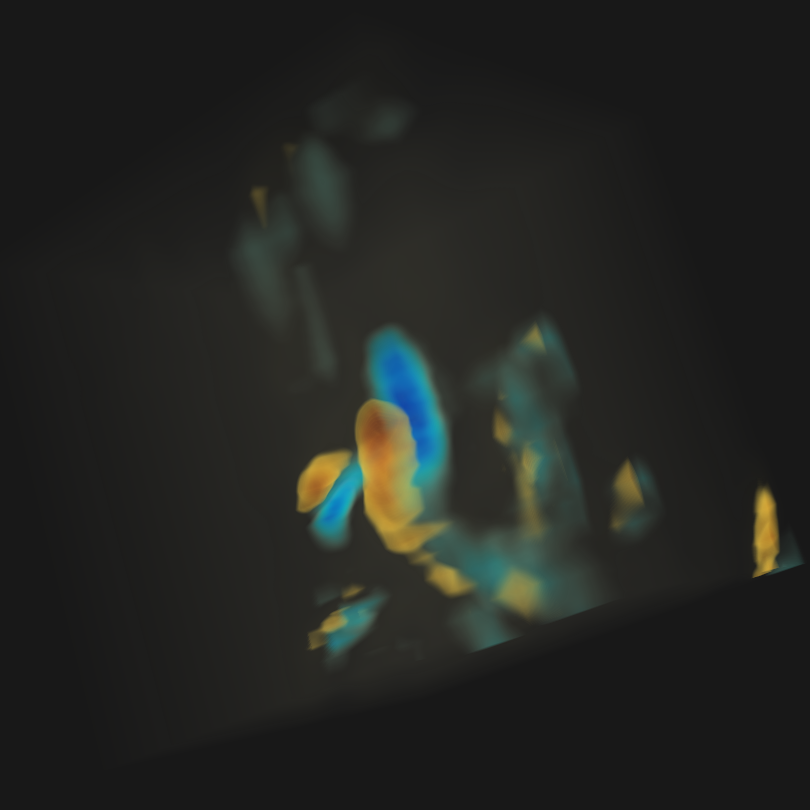
\includegraphics[width=0.31\linewidth]{gradient/gradient-turbulence-magnitude}}}
	\subcaptionbox{\emph{by signature} ($s_{grad-sig}$)}{
	{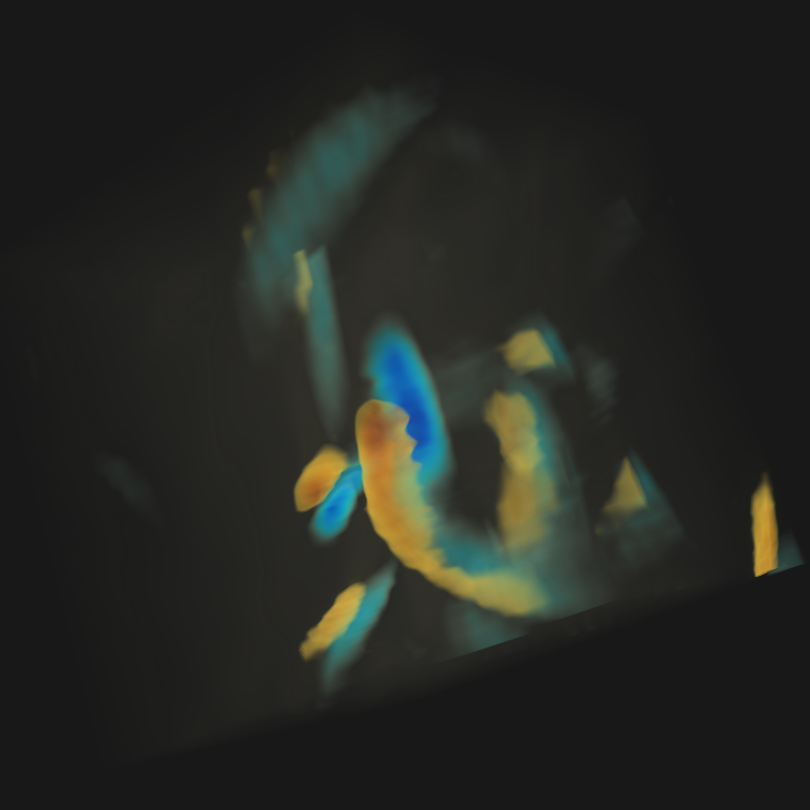
\includegraphics[width=0.31\linewidth]{gradient/gradient-turbulence-signature.png}}}
	\subcaptionbox{\emph{reference}}{
	{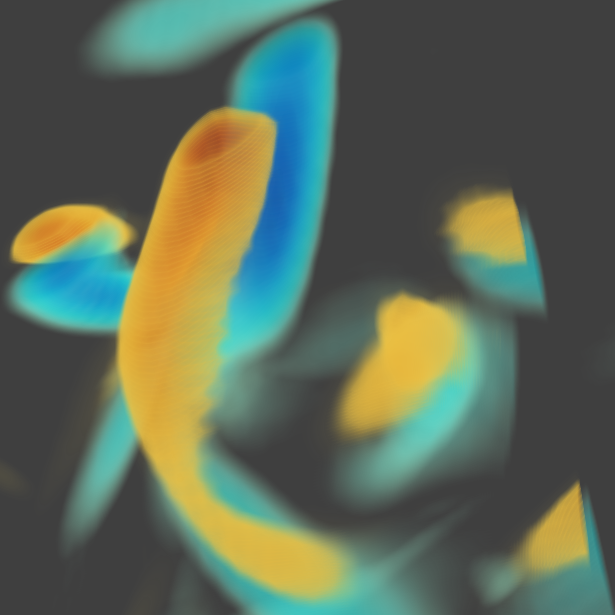
\includegraphics[width=0.31\linewidth]{gradient/gradient-turbulence-groundtruth.png}}}
	\caption{x-component of the ($64^3$) gradient field of \emph{turbulence}, reconstructed at 0.2
	bps. The gradient field produced by $s_{bit}$ is more accurate than one produced by either
	$s_{wav}$ or $s_{grad-sig}$ (compare orange features).}\label{fig:gradient-rendering-diff}
\end{figure}

For the gradient, we have experimented with three popular finite difference schemes using stencil
sizes of two, three, and five points in each dimension. We have foundno tangible differences in the
results, and therefore present results for the five-point stencil exlusively: $\frac{\partial
f}{\partial x}\approx \frac{1}{12}f(x-2)-\frac{2}{3}f(x-1)+\frac{2}{3}f(x+1)-\frac{1}{12}f(x+2)$. In
3D, the gradient at grid point $(x,y,z)$ is the vector $(\frac{\partial f}{\partial
x},\frac{\partial f}{\partial y}, \frac{\partial f}{\partial y})$. We use Algorithm~\ref{alg:greedy}
to compute a \emph{gradient-optimized} ($s_{grad-opt}$) stream that minimizes the difference between
the reconstructed gradient field and the original gradient field. The error at each grid point $x_i$
is the squared Euclidean length of the difference between two gradient vectors, that is,
$\norm{\nabla \tilde{f}(x_i)-\nabla f(x_i)}^2$, where $\tilde{f}$ is an approximation of $f$
at low bit rates. The overall error, defined over the whole field, is $e(\nabla \tilde{f},\nabla
f)=\sqrt{\frac{1}{n}\sum_{i=1}^{n}{\norm{\nabla \tilde{f}(x_i)-\nabla f(x_i)}^2}}$.

Using four data sets, we plot gradient error curves produced by $s_{lvl}$, $s_{bit}$, $s_{mag}$,
$s_{wav}$, $s_{grad-opt}$, and $s_{grad-sig}$ in \cref{fig:gradient-error-comparison}. In
general, $s_{grad-opt} > s_{grad-sig} \approx s_{bit} > s_{wav} > s_{mag} > s_{lvl}$. This ordering
can also be seen in \cref{fig:gradient-rendering-diff}, where the x-component of the gradient
field for \emph{tuburlence} is reconstructed and rendered, at 0.2 bps. Unlike in the RMSE case,
$s_{bit}$ produces better approximations of the gradient field, compared to $s_{wav}$. This
phenomenon is explained in \cref{fig:bit-plane-vs-wavelet-norm-gradient}.

In \cref{fig:bit-plane-vs-wavelet-norm-gradient}, a 1D line is extracted from \emph{plasma}, and
reconstructed using $s_{bit}$ and $s_{wav}$ at 0.6 bps. Because the coarse-scale coefficients in
$s_{bit}$ are not accurate enough, the reconstruction from $s_{bit}$ is inaccurate in areas of low
gradients. In constrast, the $s_{wav}$'s reconstruction is accurate in low-gradient areas, but lacks
the resolution to resolve the high-gradient areas. This is because $s_{wav}$ frequently intersperses
bits that improve resolution and bits that improve precision, unlike $s_{bit}$, which always stream
bits that improve resolution first. As such, $s_{wav}$ tends to produce a ``smoother''
reconstruction that, \emph{on average} (i.e., in terms of RMSE), is close to the original function.
$s_{bit}$, on the other hand, tends to capture well the function's shape (due to fine-scale bits),
but the whole function can be ``shifted'' slightly due to the lack of precision in coarse-scale
coefficients. However, the error caused by this shifting reduces significantly when taking gradient,
which cancels any constant shift. $s_{bit}$, therefore, works better than $s_{wav}$ for gradient
computation, thanks to its virtue of being able to better retain sharp features.

\duong{talk about the by-level, by-magnitude, and signature}.
\duong{explain the ``bumpiness'' in the by wavelet norm}

\subsubsection{Laplacian}\label{sec:laplacian}

\begin{figure}[h]
	\centering
	\subcaptionbox{\emph{boiler}}
	{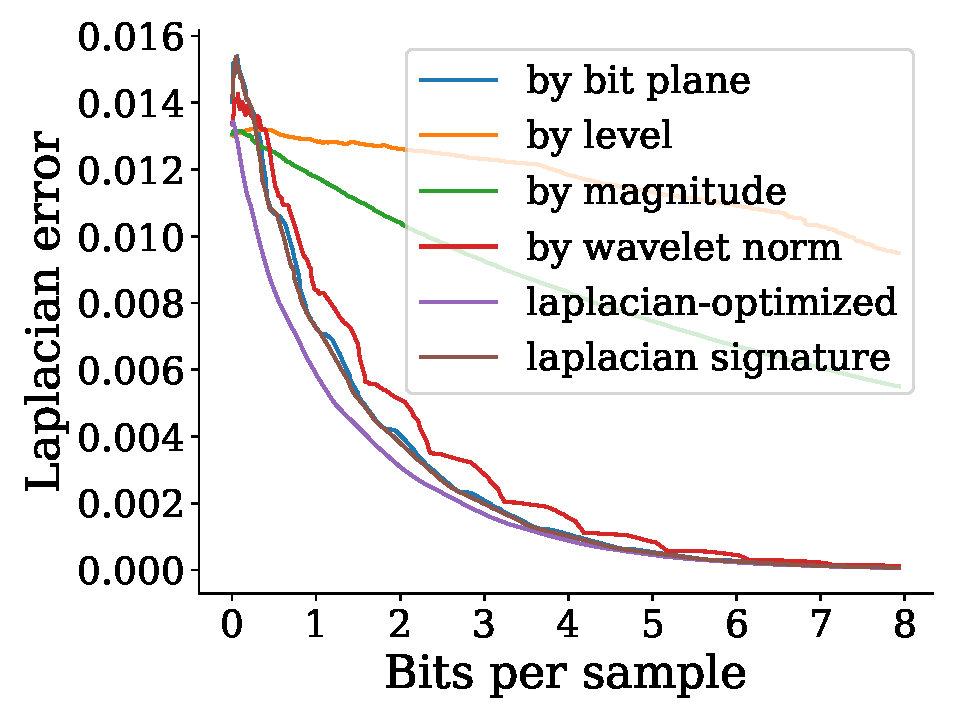
\includegraphics[width=0.48\linewidth]{laplacian/laplacian-optimized-boiler}}
	\subcaptionbox{\emph{diffusivity}}
	{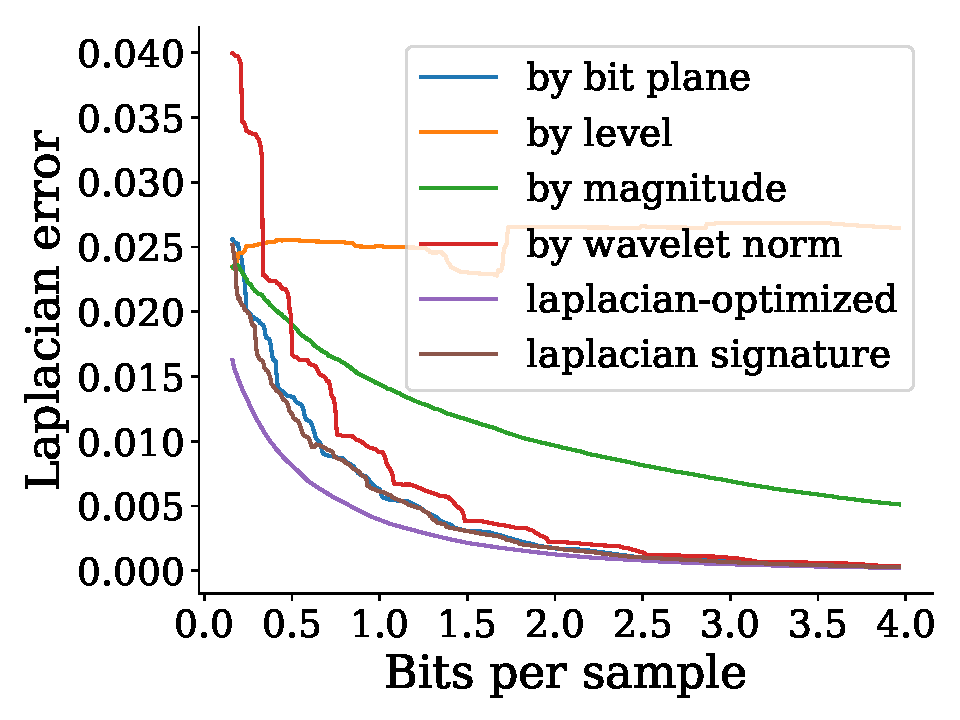
\includegraphics[width=0.48\linewidth]{laplacian/laplacian-optimized-diffusivity}}
	\subcaptionbox{\emph{turbulence}}
	{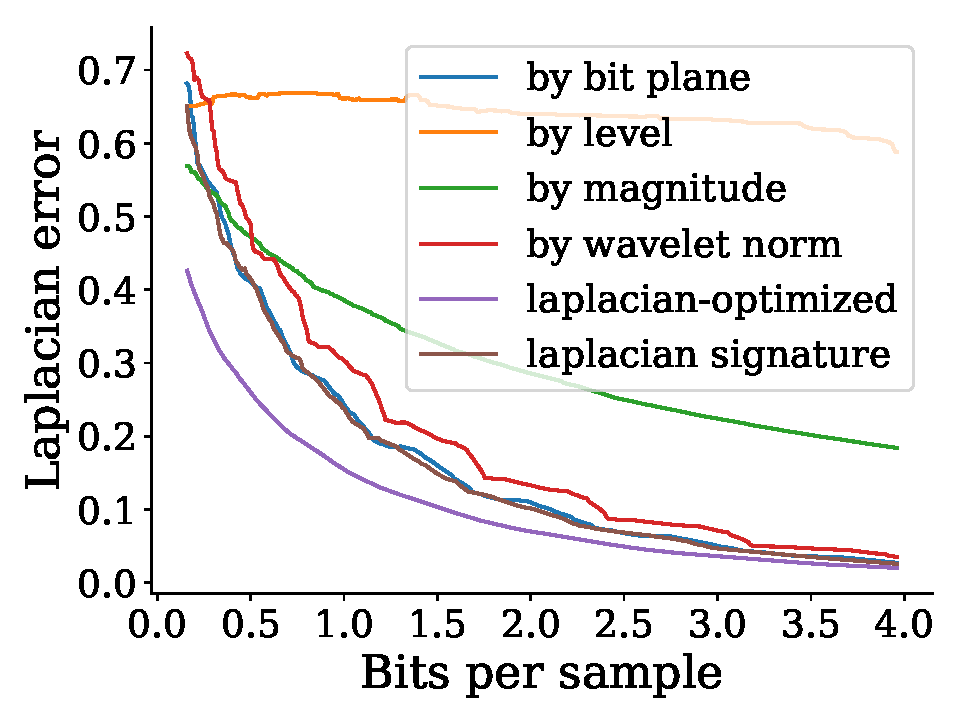
\includegraphics[width=0.48\linewidth]{laplacian/laplacian-optimized-turbulence}}
	\subcaptionbox{\emph{pressure}}
	{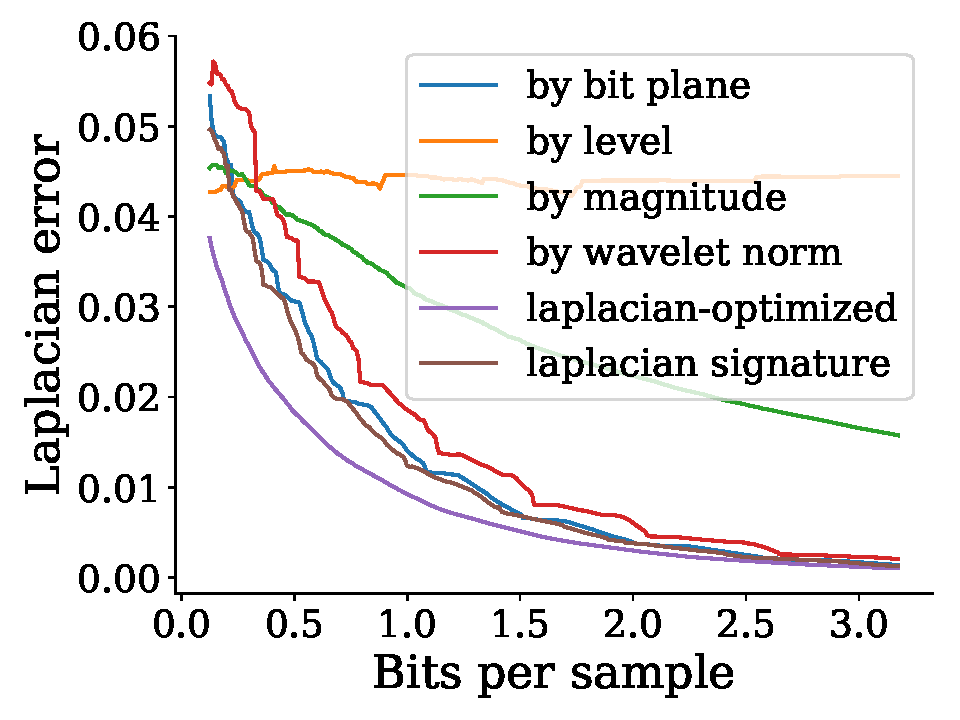
\includegraphics[width=0.48\linewidth]{laplacian/laplacian-optimized-pressure}}
	\caption{Laplacian error comparison among streams, using the three-point stencil. The plots are
	truncated so as to better highlight differences without discarding important information. In all
	cases, \emph{laplacian}}\label{fig:laplacian-error-comparison}
\end{figure}

\begin{figure}[h]
	\centering
	\subcaptionbox{\emph{by level} ($s_{lvl}$)}
	{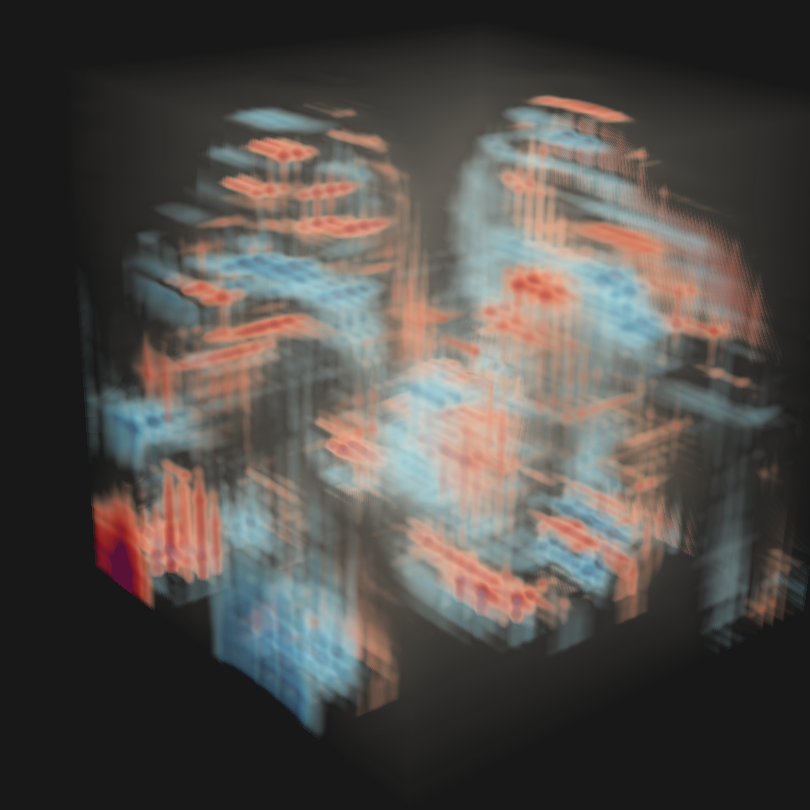
\includegraphics[width=0.31\linewidth]{laplacian/laplacian-pressure-level}}
	\subcaptionbox{\emph{by bit plane} ($s_{bit}$)}
	{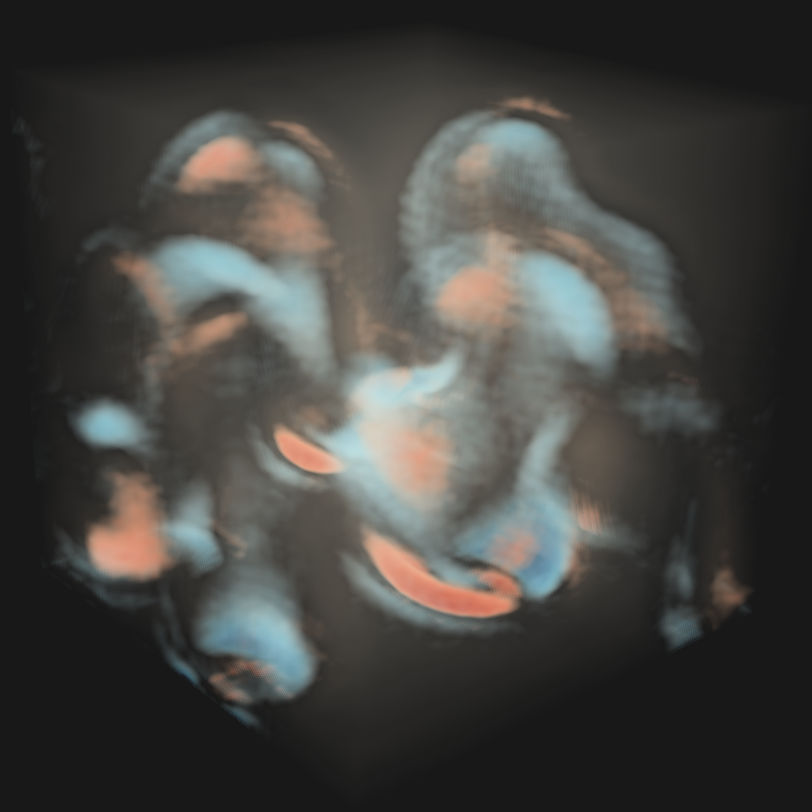
\includegraphics[width=0.31\linewidth]{laplacian/laplacian-pressure-bit-plane}}
	\subcaptionbox{\emph{by wavelet norm} ($s_{wav}$)}
	{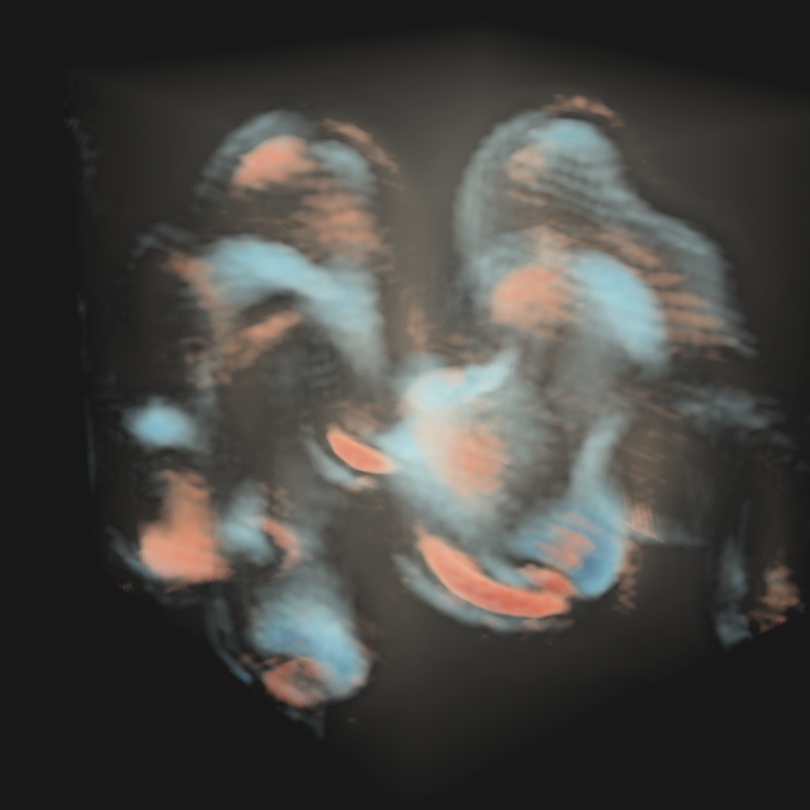
\includegraphics[width=0.31\linewidth]{laplacian/laplacian-pressure-wavelet-norm}}
	\subcaptionbox{\emph{by magnitude} ($s_{mag}$)}
	{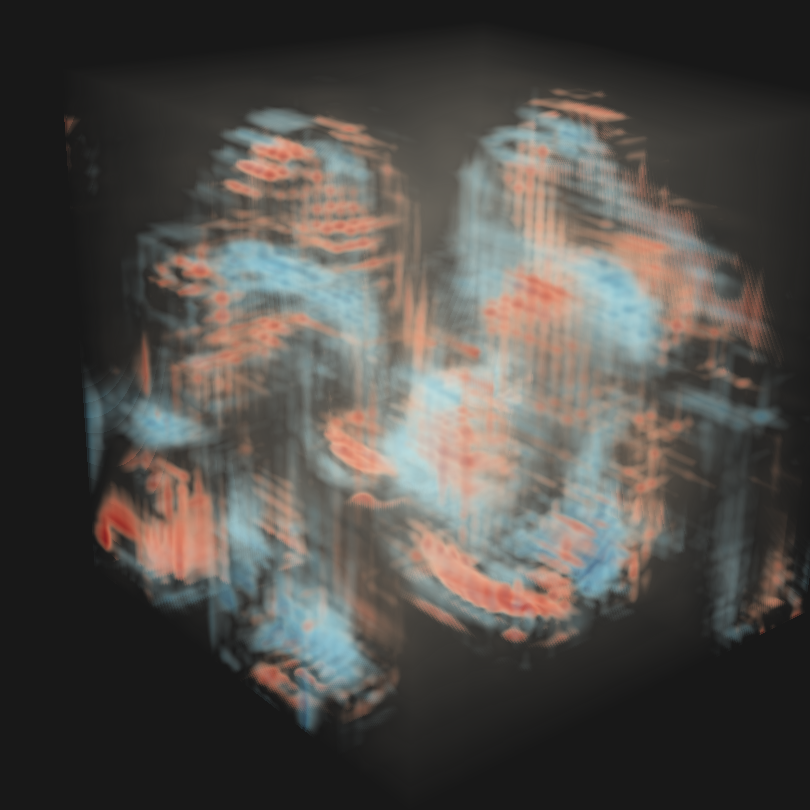
\includegraphics[width=0.31\linewidth]{laplacian/laplacian-pressure-magnitude}}
	\subcaptionbox{\emph{by signature} ($s_{lap-sig}$)}
	{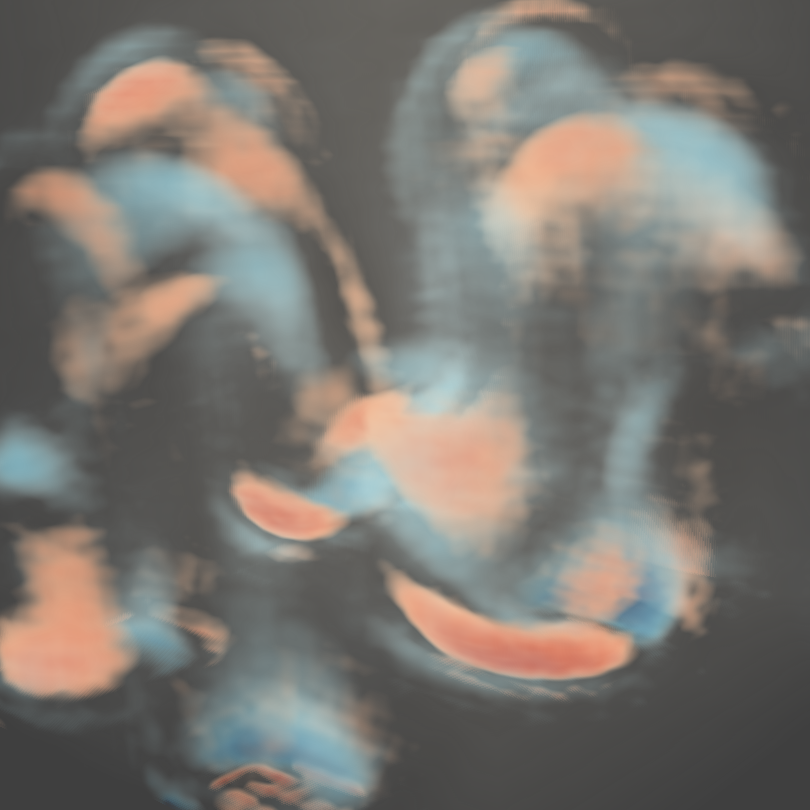
\includegraphics[width=0.31\linewidth]{laplacian/laplacian-pressure-signature}}
	\subcaptionbox{\emph{reference}}
	{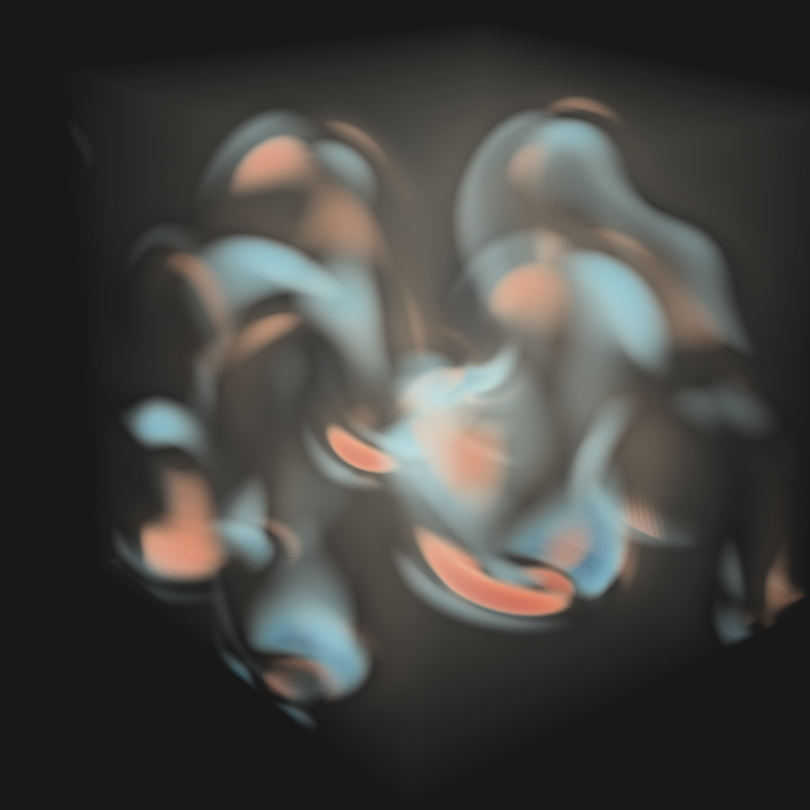
\includegraphics[width=0.31\linewidth]{laplacian/laplacian-pressure-groundtruth}}
	\caption{Renderings of recontructed Laplacian fields for a $64^3$ region in \emph{pressure}, at 0.9 bps.
	In terms of image quality, $s_{lap-sig} > s_{bit} > s_{wav} > s_{mag} > s_{lvl}$.}
	\label{fig:laplacian-renderings}
\end{figure}

\duong{give an example of where to use the LAplacian?}
The Laplace operator is a second-order differential operator, defined as the divergence of the
gradient field. It can be computed by summing second partial derivatives in all dimensions, for
example, in 3D: $\Delta
f=(\frac{{\partial}^2}{\partial{x^2}}+\frac{{\partial}^2}{\partial{y^2}}+\frac{{\partial}^2}{\partial{y^2}})f$.
It is perhaps the second-most common derivative quantity, after the gradient. To compute the
Laplacian, we use the five-point finite difference to approximate the second derivative in each
dimension: $\frac{{\partial}^2}{\partial{x^2}}f(x,y,z) \approx
-\frac{1}{12}f(x-2,y,z)+\frac{4}{3}f(x-1,y,z)+\frac{-5}{2}f(x,y,z)+\frac{4}{3}f(x+1,y,z)-\frac{1}{12}f(x+2,y,z)$.
To compare two Laplacian fields, we use the root-mean-square error, that is, $e(\Delta
\tilde{f},\Delta f)=RMSE(\Delta \tilde{f},\Delta f)$. As usual, we use Algorithm \cref{alg:greedy}
to compute a \emph{laplacian-optimized} ($s_{lap-opt}$) stream that minimizes $e$, and an
$s_{lap-sig}$ stream from its signature. \cref{fig:laplacian-error-comparison} plots the error
curves for all relevant streams. The plots here largely follow the one in
\cref{fig:gradient-error-comparison}, in terms of relative performance among the streams, with one
minor discrepancy. $s_{bit}$ consistenly underperforms $s_{lap-sig}$ by a small margin, and produces
``bumpier'' error curves. In \cref{fig:laplacian-renderings}, we render the reconstructed Laplacian
fields for the \emph{pressure} field at 0.9 bps, which shows how differences in Laplacian RMSE among
the streams translate to visual differences.
